\documentclass[11pt,a4paper]{article}
\usepackage{graphicx} % Required for inserting images
\usepackage{hyperref}
\usepackage{amsmath}
\usepackage{amsfonts}
\usepackage{amssymb}
\usepackage{makecell}
\usepackage{url}
\usepackage{xcolor}
\usepackage{multirow}
\usepackage{float}
\usepackage{amsthm}
\newtheorem{theorem}{Theorem}


\title{\textbf{A Formal Analysis of the NVIDIA PTX Memory Consistency Model}\\\Large{A Review}}

\author{
    Wuyue Sun\\
    \normalsize{\href{mailto:wuyue.sun@epfl.ch}{\texttt{wuyue.sun@epfl.ch}}}
    \and
    Boran Xu\\
    \normalsize{\href{mailto:boran.xu@epfl.ch}{\texttt{boran.xu@epfl.ch}}}
    \and
    Yue Yu\\
    \normalsize{\href{mailto:yue.yu@epfl.ch}{\texttt{yue.yu@epfl.ch}}}
}
\date{}

\begin{document}
\setlength{\parindent}{0pt}

\maketitle

\begin{abstract}
\noindent The reviewed paper \cite{10.1145/3297858.3304043} is among a series of efforts towards comprehensive GPU memory consistency modeling \cite{c11, rc11, 10.1145/3297858.3304043, 10.1145/3470496.3533045} and concurrency verification \cite{hmc, cerberus-bmc, unified}.
\end{abstract}

\section{Introduction}

\textit{\textbf{M}emory \textbf{c}onsistency \textbf{m}odel} (MCM) functions as a hardware-software contract for any shared-memory hardware architecture and programming model \cite{litmus}. A reliable MCM provides the foundation for concurrency correctness, and a weak MCM ensures high performance of concurrent programs.\\

\begin{table}[H]
\centering
\begin{tabular}{rlclll}
\multicolumn{1}{l}{} & & \multicolumn{1}{l}{} & \multicolumn{3}{c}{\multirow{2}{*}{Applications}}\\ \cline{1-3}
\multicolumn{2}{r}{\multirow{2}{*}{Libraries}} & \multicolumn{1}{c|}{} & \multicolumn{3}{c}{}\\ \cline{3-4}
\multicolumn{2}{r}{} & \multicolumn{2}{|c|}{Runtime, e.g., CUDA, OpenCL, etc.} & & \\ \cline{2-5}
\multicolumn{1}{l|}{} & \multicolumn{4}{c|}{CUDA driver} & \\ \hline
\multicolumn{3}{r}{PTX} & \multicolumn{3}{l}{\textcolor{blue}{MCM}}\\ \hline
\multicolumn{6}{c}{SASS \textcolor{gray}{(machine code)}}\\ \hline
\multicolumn{3}{r}{\textcolor{gray}{GPU} microarchitecture} & \multicolumn{3}{l}{Lower-level memory model}            
\end{tabular}
\end{table}

The NVIDIA PTX virtual \textit{\textbf{i}nstruction \textbf{s}et \textbf{a}rchitecture} (ISA) \cite{ptx} is the lowest \textbf{portable} layer of abstraction providing memory order semantics. It exposes the \textit{interfaces} to the driver, runtime, libraries, and applications to manipulate NVIDIA GPU memory access ordering.\\

\cite{10.1145/3297858.3304043} is the first to present a formal MCM industrially used by NVIDIA GPUs. The contributions of the paper are that

\begin{enumerate}
    \item it formalized MCM prose in PTX documentation to \textit{relations} and \textit{axioms};
    \item it developed a mapping from scoped C++ to PTX;
    \item it proved the soundness of such a mapping both empirically (in Alloy \cite{alloy}) and formally (in Coq \cite{coq}).
\end{enumerate}

\section{Preliminaries}

MCM is a standard that provides strong guarantees for the behavior of concurrent programs using \textit{atomic} primitives. We introduce the axiomatic approach to defining a MCM. A candidate \textit{execution} is a behavior of the concurrent program. We define an execution as a graph, whose nodes are primitive \textit{events}, and whose edges are \textit{relations}. Events include read, write, read-modify-write (RMW) \textcolor{gray}{atomics}, and fence.\\

A MCM is uniquely defined by a set of axioms. All axioms of a MCM must hold for all legal executions of a program. An axiom often expressed in terms of relations and predicates, e.g.,

$$
\verb|acyclic|(po\_loc \cup co \cup rf \cup fr)
$$

Note that $po\_loc$ denotes the \textbf{set} of all relations of type $po\_loc$ in the candidate execution; so do the other terms. The above example axiom means there is no cycle in the set of relations of type $po\_loc$, $co$, $rf$, and $fr$.

\subsection{PTX}

\begin{figure}[H]
    \centering
    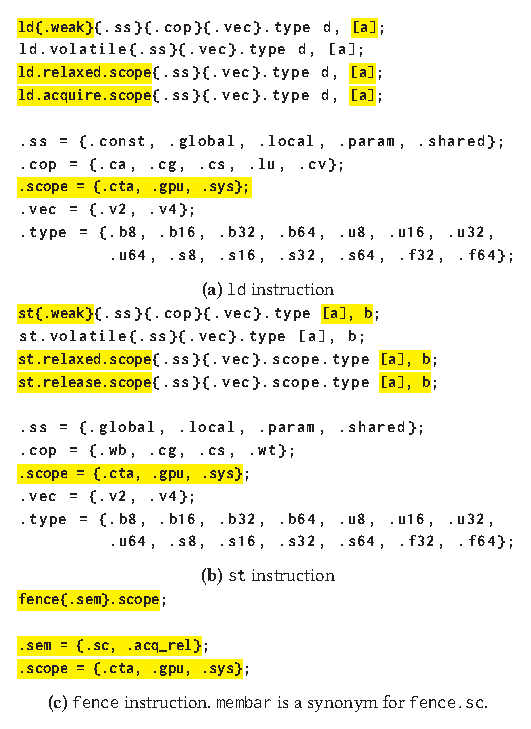
\includegraphics[width=0.75\linewidth]{img/ptx.eps}
    \caption{MCM-related PTX virtual instructions}
    \label{fig:ptx-instr}
\end{figure}

A PTX virtual instruction comprises an operation followed by various \textit{fields} and the operand(s). Fig.~\ref{fig:ptx-instr} lists the instructions concerning the PTX MCM. Only highlighted fields influence relations of events. Note, counter-intuitively, that the \textit{state space} \verb|.ss| field does not participate in MCM definition.

\subsection{x86-TSO}
\label{sec:tso}

TSO is the MCM adopted by Intel and AMD CPUs. It paves the way to PTX MCM formalization. x86-TSO comprises 2 axioms.

\begin{enumerate}
    \item \textbf{SC-per-Location}. All accesses to a memory address\footnote{The address is fixed but arbitrary.} always serialize to a \textit{total} order at runtime.
    \item \textbf{Causality} regulates memory ordering in the presence of \textit{store buffers}.
\end{enumerate}

$$
\begin{align*}
\raisebox{2.05em}{$\text{SC-per-Location} \left\{\rule{0em}{2.7em}\right.$}
    \begin{matrix}
        fr\\ 
        po\_loc\\
        rf\\
        co\\
        rfe\\
        ppo\\
        fence\\
    \end{matrix}
\raisebox{-2.05em}{$\left.\rule{0em}{2.7em}\right\} \text{Causality}$}
\end{align*}
$$

Above lists the relations used by each axiom. We omit the exact definition of x86-TSO MCM axioms.

\section{PTX MCM formalism}

PTX MCM is \textbf{non}-multi-copy atomic, which does not enforce the \textit{data race free} (DRF) property on programs.

\subsection{Relations}

Compared to \ref{sec:tso}, PTX MCM additionally (modifies and) defines the following relations.

\begin{enumerate}
    \item \textbf{Synchronizes-with ($sw$)}. This is also known as the \textit{release consistency} order, which involves 3 components: release pattern $pattern_{rel}$, observation $obs$, and acquire pattern $pattern_{acq}$.\\

    The PTX documentation defines \textit{morally strong} in \href{https://docs.nvidia.com/cuda/parallel-thread-execution/index.html#morally-strong-operations}{\S8.7}. A write W precedes a read R in $obs$ either
    
    \begin{itemize}
        \item W and R are mutually strong, and R $\xrightarrow[]{rf}$ W; or
        \item for some atomic operation Z, W $\xrightarrow[]{obs}$ Z $\xrightarrow[]{obs}$ R
    \end{itemize}

    Note the \textbf{recursive} definition.
    \item \textbf{Barrier} synchronization have a similar effect to the release-acquire pattern, but at a \verb|.cta| scope.
    \item \textbf{Fence-SC ($sc$)} relates every pair of morally strong \verb|fence.sc| operations.
    \item \textbf{Base causality ($cause_{base}$)} results from the combination of $po$ and $sw$. For 2 operations X and Y, X $\xrightarrow[]{cause}$ Y $\displaystyle \triangleq$

    \begin{itemize}
        \item X $\xrightarrow[]{sw}$ Y; or
        \item for some operation Z,
        
        \begin{itemize}
            \item X $\xrightarrow[]{po}$ Z $\xrightarrow[]{cause}$ Y; or
            \item X $\xrightarrow[]{cause}$ Z $\xrightarrow[]{po}$ Y; or
            \item X $\xrightarrow[]{cause}$ Z $\xrightarrow[]{cause}$ Y
        \end{itemize} 
    \end{itemize}
\end{enumerate}

\subsection{Axioms}

Given the above relations, PTX MCM enforces the following axioms.


\begin{table}[H]
    \centering
    \begin{tabular}{c|ccc}
        \textbf{Axiom} & \textbf{Name} & \textbf{Formula} & \textbf{Description}\\
        \hline
        1 & Coherence & [W]; $cause$; [W] $\subseteq co$ & \makecell[l]{Partial transitive order\\relating overlapped writes}\\
        \hline
        2 & FenceSC & \verb|irreflexive|($sc$; $cause$) & \makecell[l]{FenceSC does not contradict\\Causality.}\\
        \hline
        3 & Atomicity & \makecell[r]{$\texttt{empty}\Big(\big((morally\_strong~\cap$\\$rf); (morally\_strong \cap co)\big)$\\$\cap~rmw\Big)$} & \makecell[l]{RMW instr. are atomic.}\\
        \hline
        4 & No-Thin-Air & $\verb|acyclic|(rf \cup dep)$ & \makecell[l]{No ``out of thin air" bug}\\
        \hline
        5 & SC-per-Location & \makecell[r]{$\texttt{acyclic}\Big(\big(morally\_strong$\\$\cap~(rf \cup co \cup fr)\big) \cup po\_loc\Big)$} & \makecell[l]{Morally strong communication\\order cannot contradict\\program order.}\\
        \hline
        6 & Causality & \makecell[r]{$\texttt{irreflexive}\big((rf \cap fr);$\\$cause\big)$} & \makecell[l]{Communication order cannot\\contradict base causality.}\\
    \end{tabular}
    \caption{Axiomatic MCM of PTX}
    \label{table:axiom}
\end{table}

A \textit{consistent} execution \textbf{must} satisfy the above axioms.

\section{Scoped C++ to PTX mapping}

\begin{figure}[H]
    \centering
    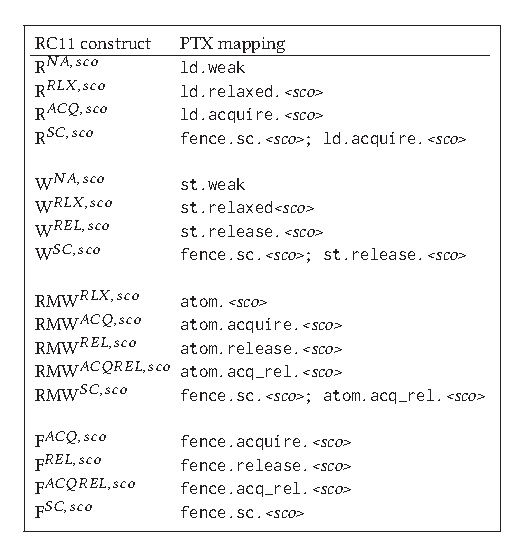
\includegraphics[width=0.75\linewidth]{img/mapping.eps}
    \caption{Mapping from extended RC11 \cite{rc11} to PTX}
    \label{fig:mapping}
\end{figure}

The formal PTX MCM serves as a target for a language\footnote{Example languages are CUDA C++, OpenCL, and Fortran.}-level memory model that compiles onto PTX. \cite{10.1145/3297858.3304043} provided a mapping from the high-level MCM to PTX in Fig.~\ref{fig:mapping} and verified its soundness. The paper extended the RC11 MCM \cite{rc11} with the notion of \textit{scope}.\\

We do not elaborate further because this part does not concern our project.

\section{Analyzing PTX Using Alloy and Coq}

Alloy \cite{alloy} is a \textbf{d}omain \textbf{s}pecific \textbf{l}anguage (DSL) to describe and empirically test relational models. Using the syntax of Alloy, the memory model of PTX and scoped C++ can be easily expressed. The paper also encoded the mapping into Alloy.\\

The paper then presented a theorem that states the correctness of the mapping from scoped C++ to PTX. According to the theorem, \textbf{given} a legal execution $e'$ of a PTX program $p'$ --- translated from a C++ program $p$ by Fig.~\ref{fig:mapping} --- \textbf{if} we interpret $e'$ as an execution $e$ of the original C++ program $p$, \textbf{then} $e$ is a legal execution of $p$. This theorem establishes the equivalence between scoped RC11 and PTX MCM.\\

The theorem was proven by Coq \cite{coq} with the help of an Alloy-to-Coq compiler, \verb|alloyqc|. It translates the Alloy MCM specifications to Coq, along with its associated theorems. This provides a basis on which the user can fill in the proofs. This compiler support any model; however, its primary use in the paper was to verify the soundness of the scoped-C++-to-PTX mapping \textcolor{gray}{rather than concurrent programs}.

\section{Results of Testing and Verifying the Mapping from Scoped C++ to PTX}

The authors evaluated two versions of the scoped C++ to PTX mapping: a standard version and a ``de-scoped" version, which omitted scopes. Adding scopes significantly increased analysis time, corroborating previous findings that memory model analysis time ``escalates exponentially with model size." A bound of five to six events was not able to uncover all \textit{litmus tests} \cite{litmus}, suggesting improvements to more refined modeling or advanced solver techniques.\\

Empirical testing missed counter-examples demonstrating ``holes" of the mapping. Due to the time complexities involved, empirical testing is complemented by formal correctness proof. Machine checked Coq proof is presented as a supplement\footnote{\url{https://github.com/nvlabs/ptxmemorymodel}} that proves the following theorems:

\begin{enumerate}
    \item RC11 Coherence is satisfied;
    \item RC11 Atomicity is satisfied;
    \item RC11 SC is satisfied.
\end{enumerate}


\section{Conclusion}

The paper contributes to the domain of formally defined memory model in several ways. First, it provided an axiomatic description of the PTX 6.0 MCM, which was previously only described in prose. Second, it conducted a formal axiomatic analysis on the model, thereby proving the validity of it. Third, the paper proposed a mapping from a scoped C++ memory model to the PTX MCM and expressed both the mapping and the models in Alloy. Finally, using a new Alloy-to-Coq compiler, \verb|alloyqc|, the paper proved the correctness of the mapping. This work underscores the suitability of the PTX memory model as a target for higher-level languages.\\

We highlight the novelty of this paper for its focus on an unconventional topic. While efforts have been made to formalize MCM for high-level programming languages, an \textit{intermediate representation}\footnote{PTX is an IR in essence even if it is called a \textbf{virtual} ISA. Unlike CPUs, GPU machine code does not provide backward compatibility.} (IR) like PTX has rarely been the target of axiomatic analysis. A formally verified MCM at this level of abstraction could provide a solid foundation for verifying higher-level memory models.


\subsection{Connections to the project}

Given the MCM provided by the paper, we trust the following parts.

\begin{enumerate}
    \item The mapping from \textbf{CUDA} to PTX, performed by NVIDIA CUDA compiler \verb|nvcc|, is sound.
    \item There is no ``hole" in PTX MCM.
    \item The mapping from PTX to SASS, performed by \verb|nvcc|, is sound.
    \item The GPU correctly implements a lower-level MCM in hardware.
\end{enumerate}

We plan to verify the correctness of a multi-GPU barrier synchronization\footnote{The code was already submitted in our proposal.}. We will first compile the \textit{kernel} to PTX. We will then describe its executions \textbf{in Alloy}. Finally, we propose to empirically verify memory access safety of the code snippet with Alloy. The plan for the \textit{150\%} goal is omitted.

\bibliographystyle{acm}
\bibliography{ref.bib}

\end{document}
